\documentclass[oneside, a5paper,10pt]{article}
\usepackage[utf8]{inputenc}
\usepackage[T2A]{fontenc}
\usepackage[russian]{babel}
\usepackage{amsmath, amssymb}
\usepackage{geometry}
\geometry{top=1.2cm, bottom=1.2cm, left=1.2cm, right=1.2cm}
\usepackage{graphicx}
\usepackage{caption}
\usepackage{float}
\captionsetup{font=small}
\pagenumbering{gobble}


\title{\textbf{Влияние формулировки задачи на решение методом PINN}}
\author{Донецков Андрей Дмитриевич$^{1,*}$, Бакакин Валерий Дмитриевич$^1$, \\ Жулев Егор Михайлович$^1$ \\
\small $^1$НИЯУ МИФИ\\
\small $^*$e-mail: andrey.donetskov@gmail.com}
\date{}

\begin{document}
\maketitle

\section*{Аннотация}
Целью работы является анализ влияния различных формулировок задачи Коши для уравнения гармонического осциллятора с вынуждающей силой на эффективность и точность решений. Проведённые эксперименты показали влияние постановки задачи на сходимость нейронной сети и вычислительные затраты.

\textbf{Ключевые слова:} гармонический осциллятор, PINN.

\section*{Постановка задачи}
Рассматриваются три постановки задачи Коши:

\textbf{1. ОДУ второго порядка:}
\begin{equation}
\frac{d^2x}{dt^2} + \omega_0^2 x = -A\cos(\omega t), \quad x(0) = x_0, \quad \frac{dx}{dt}(0) = v_0.
\end{equation}

\textbf{2. Система ОДУ первого порядка:}
\begin{equation}
\frac{dx}{dt} = y, \quad \frac{dy}{dt} = -\omega_0^2 x - A\cos(\omega t), \quad x(0) = x_0, \quad y(0) = v_0.
\end{equation}

\textbf{3. Альтернативная система ОДУ:}
\begin{equation}
\frac{dx}{dt} = \omega y - \frac{A}{\omega} \sin(\omega t), \quad \frac{dy}{dt} = -\omega x, \quad x(0) = x_0, \quad y(0) = \frac{v_0}{\omega}.
\end{equation}

\section*{Методология}
Физически-информированные нейронные сети (PINN) используются для аппроксимации решений.~\cite{raissi2019} Функция потерь минимизирует отклонения от исходных уравнений и начальных условий.~\cite{lagaris1998}

\section*{Результаты}
\begin{figure}[H]
    \centering
    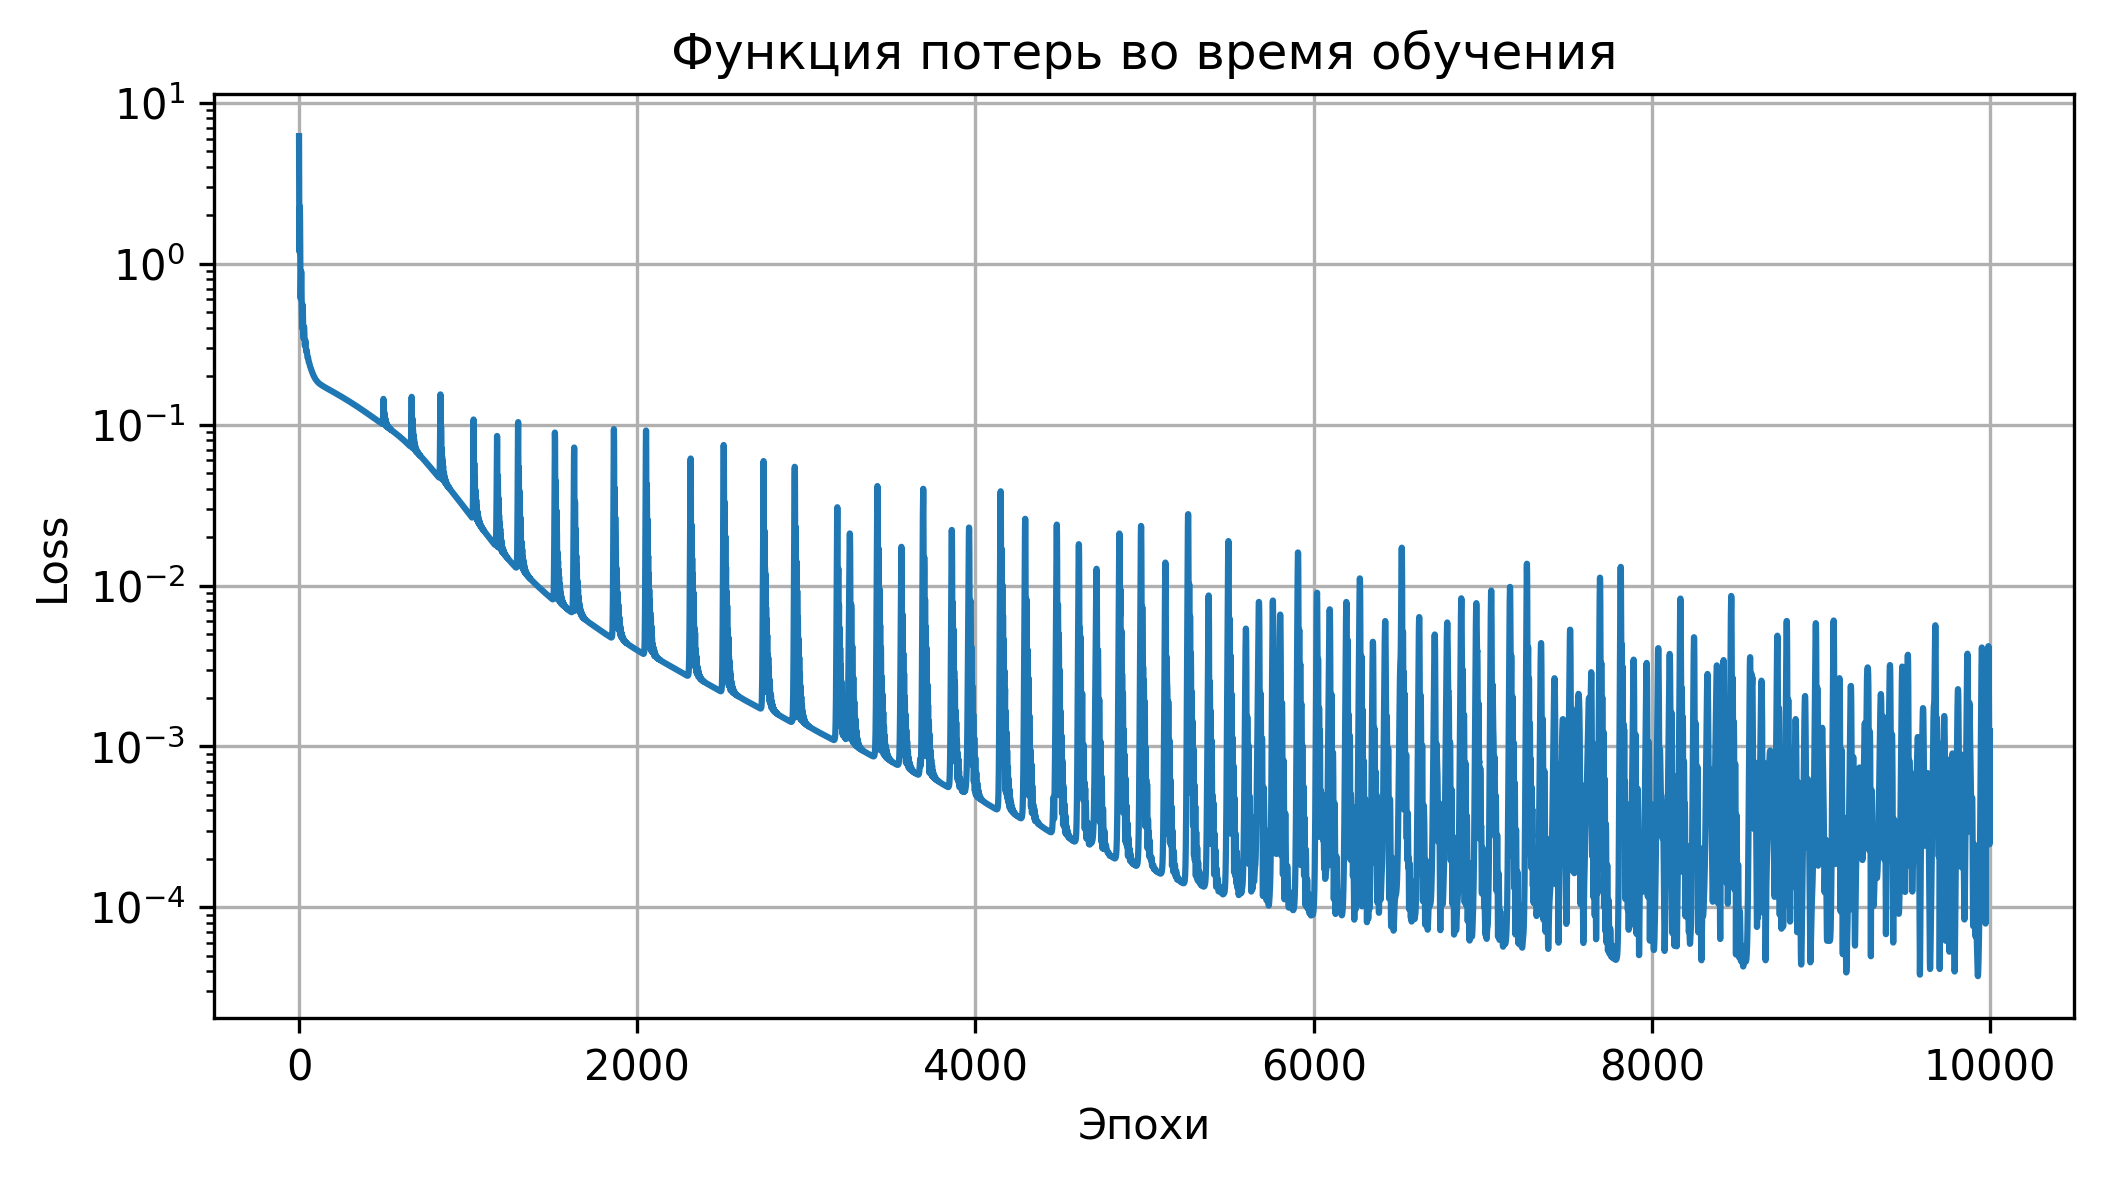
\includegraphics[width=0.3\textwidth]{../images/Loss_alt_ODE.png}
    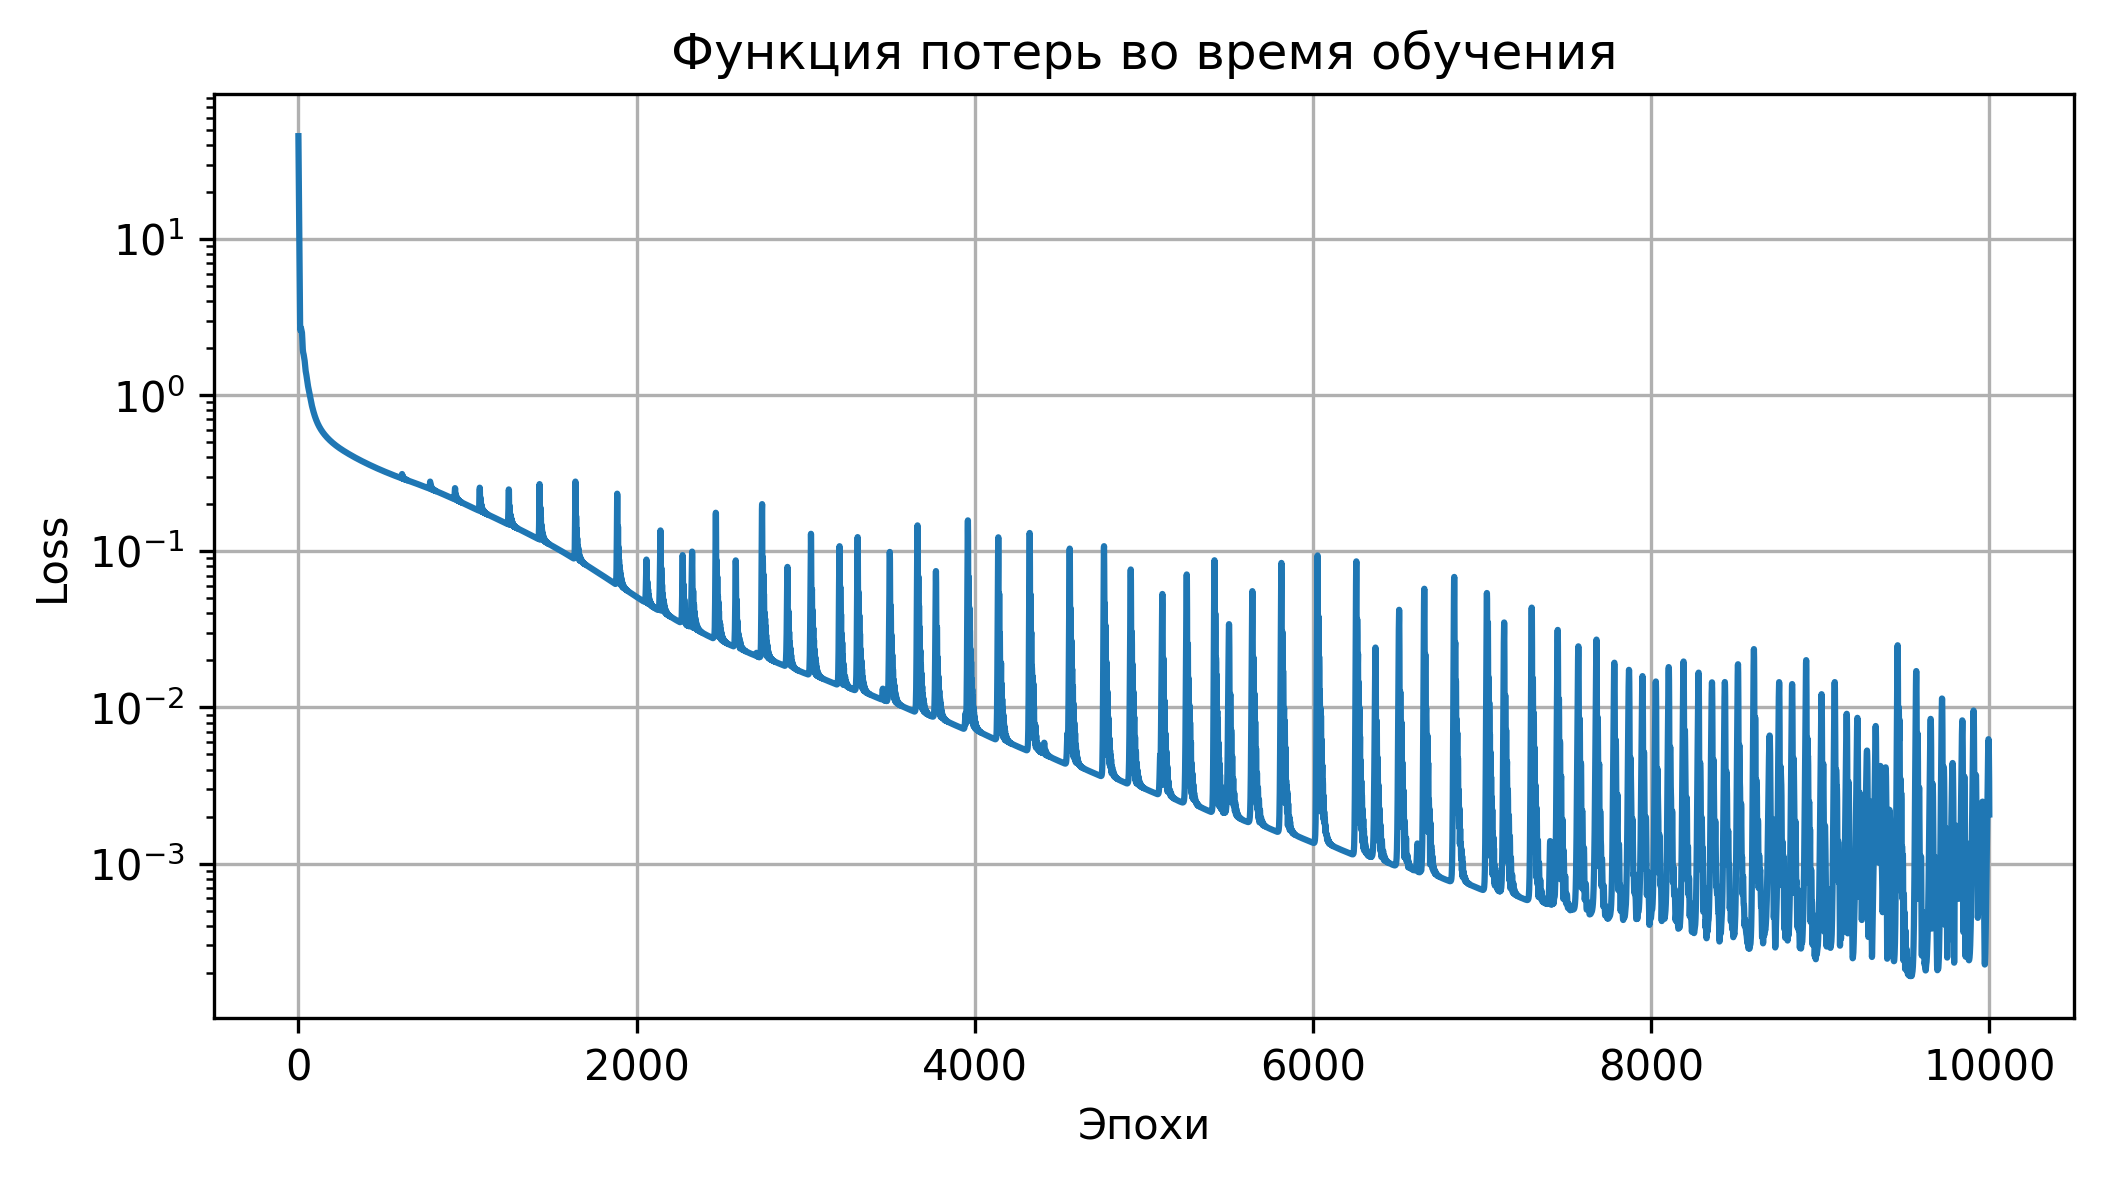
\includegraphics[width=0.3\textwidth]{../images/Loss_ODE_of_the_first_order.png}
    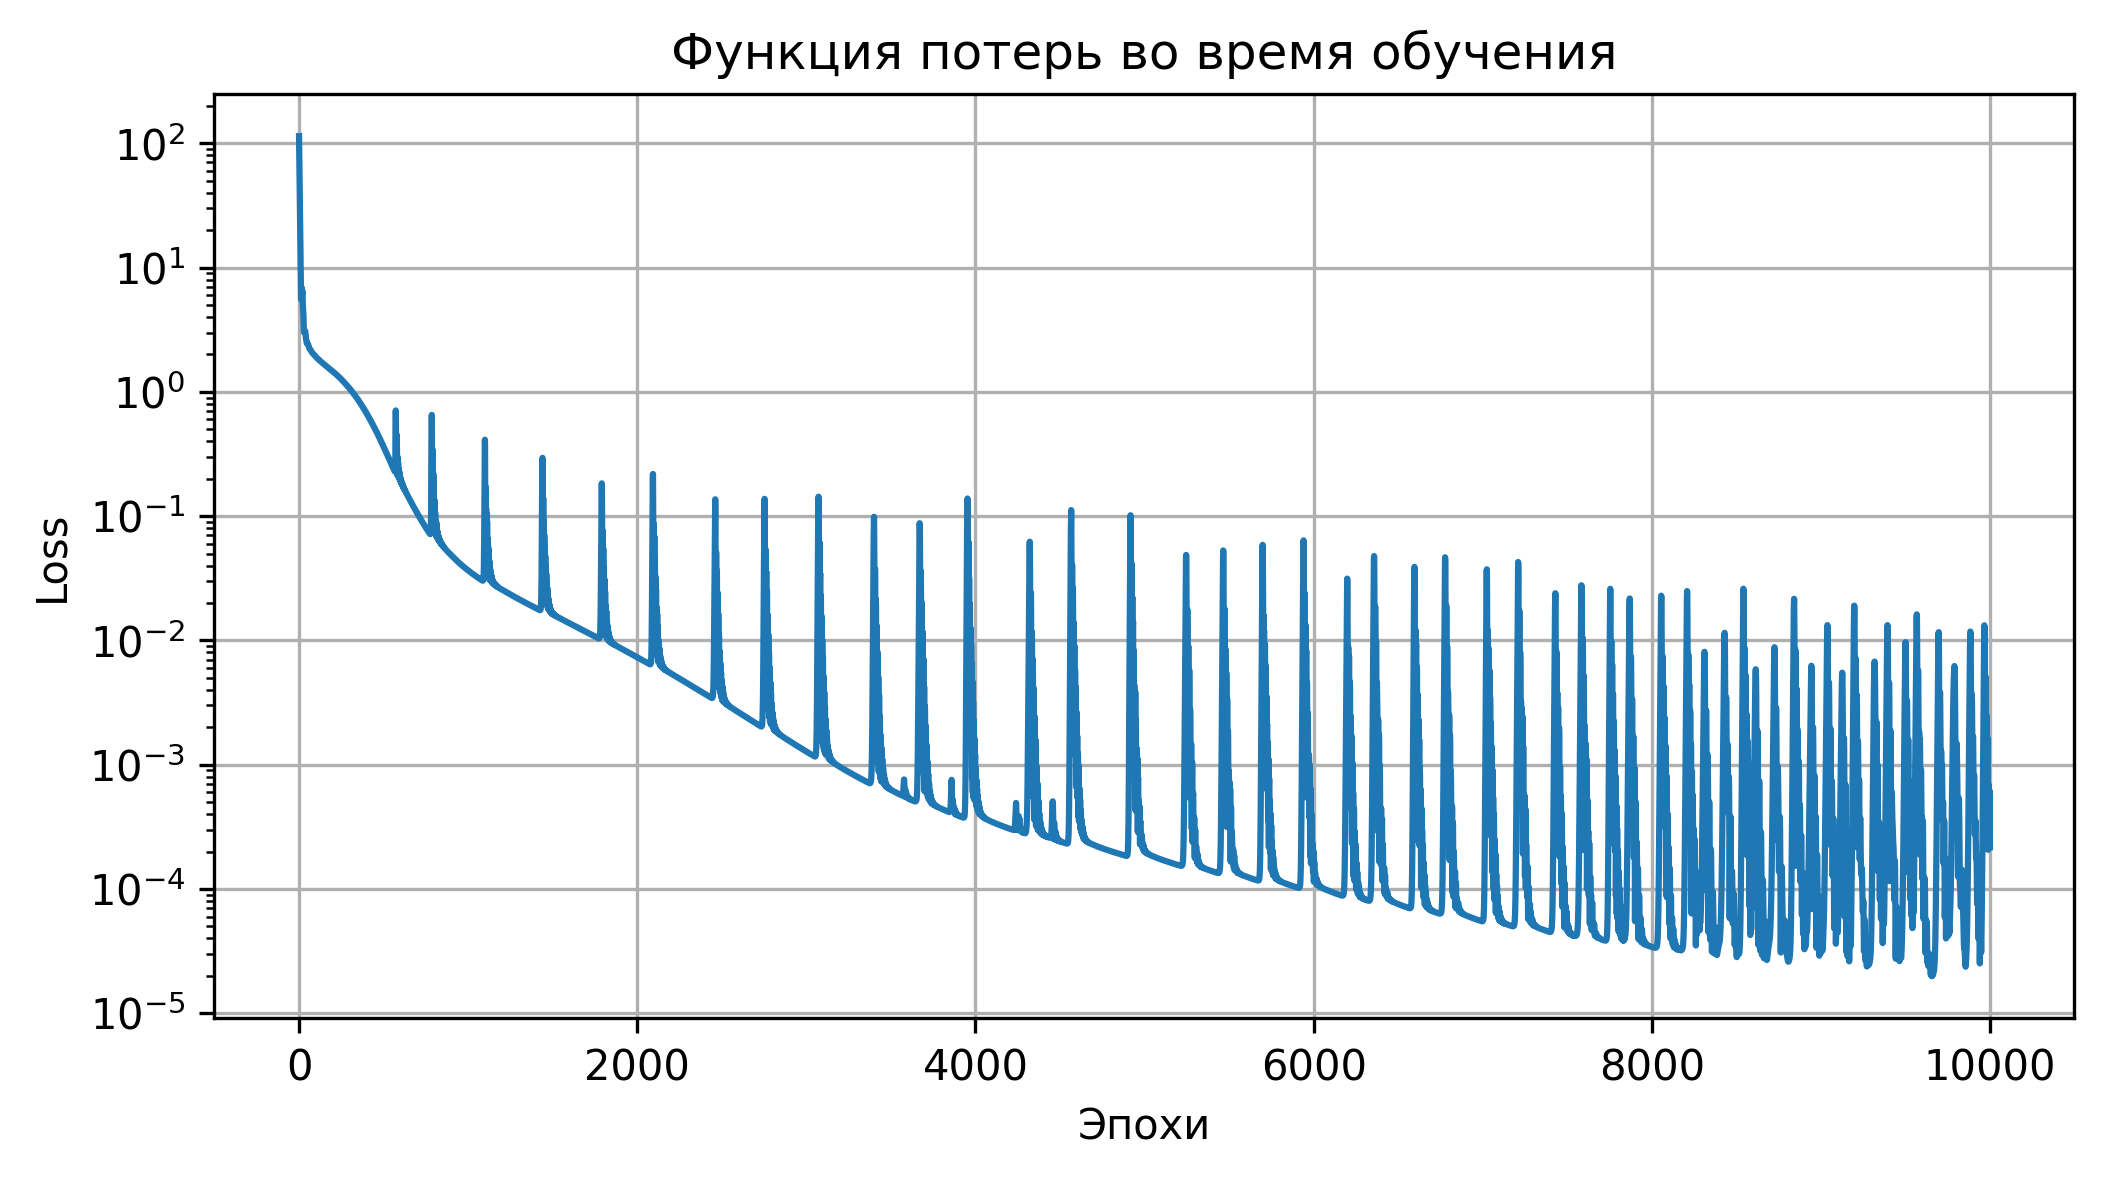
\includegraphics[width=0.3\textwidth]{../images/Loss_ODE_of_the_second_order.png}
    \caption{Функция потерь для альтернативной системы (слева), системы ОДУ первого порядка (в центре) и второго порядка (справа).}
\end{figure}

Анализ графиков функции потерь показывает, что:
\begin{itemize}
    \item \textbf{ОДУ второго порядка} показывает наибольшую скорость сходимости и высокую точность, но часто выходит из локальных минимумов;
    \item \textbf{Система ОДУ первого порядка} показывает медленную скорость сходимости и меньшую точность, но процесс обучения довольно стабилен;
    \item \textbf{Альтернативная система ОДУ} показывает точность сопоставимую с первой при меньших колебаниях loss - функции.
\end{itemize}

Таким образом, выбор формулировки задачи существенно влияет на характер сходимости и вычислительные затраты.

\begin{thebibliography}{9}
    \bibitem{lagaris1998} Lagaris I.E., Likas A., Fotiadis D.I. Artificial neural networks for solving ordinary and
    partial differential equations //IEEE transactions on neural networks. — 1998. — Т. 9. — №. 5. — С. 987-1000.
    \bibitem{raissi2019} Raissi M., Perdikaris P., Karniadakis G.E. Physics-informed neural networks: A deep
    learning framework for solving forward and inverse problems involving nonlinear partial
    differential equations //Journal of Computational Physics. — 2019. — Т. 378. — С. 686-
    707.
\end{thebibliography}

\end{document}
